\section{Context-aware Systems}
Context-aware systems are ones that are able to adapt their behavior according to changing circumstances without user intervention.
% A \emph{reflective system} is a system which incorporates structures representing (aspects of) itself. A \emph{causal connection} between a model and a element modeled exists if one of them changes, this leads to a corresponding effect upon the other~\cite{maes_concepts_1987}.

\cite{finkelstein_framework_2001} describe a framework for context-aware services.

\begin{figure}[!htb]
  \centering
  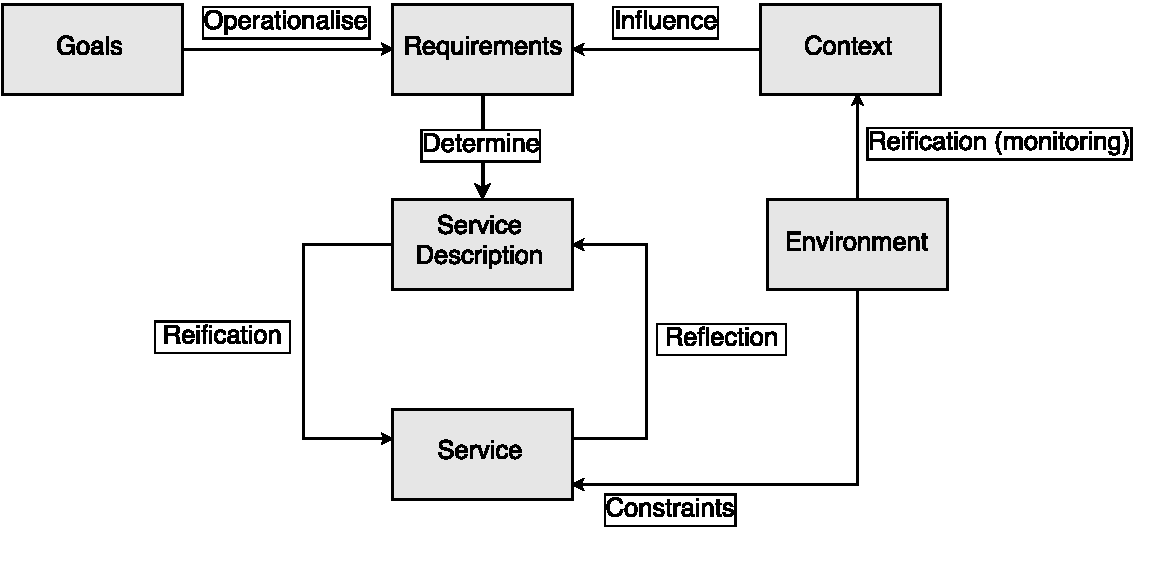
\includegraphics[width=\linewidth]{finkelstein_framework}
  \caption{Context-aware services framework by~\cite{finkelstein_framework_2001}}
\label{fig:finkelstein_framework}
\end{figure}

Goal is an objective the system should achieve. It is an abstract and long term objective.

Environment is whatever in the world provides a surrounding in which the agent is supposed to operate. The environment comprise such things as characteristics of the device that the agent is supposed to operate in.

Context is the reification of the environment. The context provides a manageable, easily computer manipulable description of the environment. A context-aware system should watch relevant environment properties and keep a runtime model that represents that information. By reasoning about that model the system can change its behavior. A context can be either a activator of goals or a precondition on the applicability of certain strategy to reach a goal.

A requirement operationalises a goal. It represents a more concrete, short-term objective that is directly achievable through actions performed by one or more agents.

Service description is the meta-level representation of the actual, real-world service. It should be a suitable formalism that allows services to be compared to requirements in order to identify runtime violations.

Service provides the actual behavior as perceived by the user.

The system should keep a causal connection between the service and the description. The system adapts by manipulating the service description.

% Requirements reflection was also proposed~\cite{bencomo_requirements_2010} as a way of drive system adaptation.
